%\documentclass[twocolumn,showpacs,preprintnumbers,amsmath,amssymb,aps,prb,floatfix]{revtex4-1}
\documentclass[preprint,showpacs,preprintnumbers,amsmath,amssymb,aps,prb,floatfix]{revtex4-1} %twocolumn,
%\documentclass[preprint,floatfix,aps,prb]{revtex4-1}
\usepackage{amssymb}
\usepackage{amsmath}
\usepackage{graphicx}
\usepackage{dcolumn}
\usepackage{bm}
\usepackage[latin1]{inputenc}
\usepackage[active]{srcltx}%habilita a pesquisa inversa
\usepackage{ae,aecompl}
\usepackage{color}
%\usepackage{pslatex}
%\usepackage[T1]{fontenc}
%\AtBeginDocument{\RequirePackage{lmodern, times}}
%\setcounter{MaxMatrixCols}{1000}
%TCIDATA{OutputFilter=Latex.dll}
%TCIDATA{Version=5.50.0.2890}
%TCIDATA{<META NAME="SaveForMode" CONTENT="1">}
%TCIDATA{BibliographyScheme=BibTeX}
%TCIDATA{LastRevised=Wednesday, February 08, 2012 17:46:00}
%TCIDATA{<META NAME="GraphicsSave" CONTENT="32">}

\newcommand{\delneg}{\boldsymbol{\delta}}
\newcommand{\signeg}{\boldsymbol{\sigma}}
\newcommand{\sigmal}{\sigma^{\prime}}
\newcommand{\sigmall}{\sigma^{\prime\prime}}
\newcommand{\xneg}{\textbf{x}}
\newcommand{\yneg}{\textbf{y}}
\newcommand{\vneg}{\textbf{v}}
\newcommand{\zneg}{\textbf{z}}
\newcommand{\knegl}{\textbf{k}^{\prime}}
\newcommand{\xnegl}{\textbf{x}^{\prime}}
\newcommand{\kneg}{\textbf{k}}
\newcommand{\apotvetor}{\textbf{A}}
\newcommand{\pneg}{\textbf{p}}
\newcommand{\lneg}{\textbf{l}}
\newcommand{\pnegl}{\textbf{p}^{\prime}}
\newcommand{\qneg}{\textbf{q}}
\newcommand{\qnegl}{\textbf{q$^{\prime}$}}
\newcommand{\rneg}{\textbf{r}}
\newcommand{\rnegl}{\textbf{r$^{\prime}$}}
\newcommand{\rnegll}{\textbf{r$^{\prime\prime}$}}
\newcommand{\kum}{\kneg_{1}}
\newcommand{\kdois}{\kneg_{2}}
\newcommand{\sigum}{\sigma_{1}}
\newcommand{\sigdois}{\sigma_{2}}
\newcommand{\sop}{\textbf{S}}
\newcommand{\bra}{\langle}
\newcommand{\ket}{\rangle}
\newcommand{\vermelho}[1]{\textcolor{red}{#1}}
%\input{tcilatex}
\begin{document}
%\singlespacing


%\maketitle
%\thispagestyle{empty}
%\tableofcontents

%\input{abstract}
%\section{PHYSICAL REVIEW B 93, 235440 (2016)\\Section II-A \& Appendix B}

Here we follow the reference and define the following matrix $\mathbf{L}$ relating the current densities and the the corresponding values of the chemical potencial at each terminal. We are assuming here the system composed by three terminals with one of them being superconductor. 


In the linear regime response, $J_{i}$ is the current density which is given by Eq. (2) of the paper, reproduced below:
\begin{align}\label{Ji}
J_{i}=\sum_{j\neq i}\mathcal{L}_{ij,\mu}\Delta\mu_{ij}+\sum_{j\neq i}\mathcal{L}_{ij,T}\Delta T_{ij,}
\end{align}
with
$eV_{ij}=\Delta\mu_{ij}=\delta\mu_{i}-\delta\mu_{j}$, $\Delta T_{ij}=\delta T_{i}-\delta T_{j}$. The authors assume $\vec{B}=0$ and time-reversal symmetry which lead to the symmetry of the kinectic coefficients $\mathcal{L}_{ij,\mu}=\mathcal{L}_{ji,\mu}$ and $\mathcal{L}_{ij, T}=\mathcal{L}_{ji,T}$.


\subsection{Isothermal conditions --- step \#1}

In order to demonstrate some of the equations appearing in the paper, I shall start from the general expression:
\begin{align*}
\begin{bmatrix}
J_{L}
\\
J_{S}
\\
J_{R}
\end{bmatrix}
=
\begin{bmatrix}
0 & \mathcal{L}_{LS,\mu} & \mathcal{L}_{LR,\mu}
\\
\mathcal{L}_{SL,\mu} & 0 & \mathcal{L}_{SR,\mu}
\\
\mathcal{L}_{RL,\mu} & \mathcal{L}_{RS,\mu} & 0
\end{bmatrix}
\begin{bmatrix}
\delta\mu_{L}
\\
\delta\mu_{S}
\\
\delta\mu_{R}
\end{bmatrix}
\end{align*}
where we assuming the isothermal condition, which is stated in the paper. In addition, the diagonal terms are zero since the summation is over different indexed as shown in Eq. [1] of the paper.

We need to invert such equations in order to write the chemical potencial in terms of the current densities. Thus, we have:
\begin{align*}
\delta\vec{\mu}=\boldsymbol{\mathcal{L}}_{\mu}^{-1}\vec{J}
\end{align*}
% \begin{widetext}
% \begin{align*}
% \boldsymbol{\mathcal{L}}_{\mu}^{-1}=\dfrac{1}{D_{\mu}}\left[
% \begin{smallmatrix}
% \mathcal{L}_{RS,\mu} \mathcal{L}_{SL,\mu}+\mathcal{L}_{LR,\mu} \left(\mathcal{L}_{SL,\mu}+\mathcal{L}_{SR,\mu}\right) & \mathcal{L}_{LS,\mu} \mathcal{L}_{RS,\mu}+\mathcal{L}_{LR,\mu}
% \left(\mathcal{L}_{LS,\mu}+\mathcal{L}_{RS,\mu}\right) & \mathcal{L}_{LS,\mu} \mathcal{L}_{SR,\mu}+\mathcal{L}_{LR,\mu} \left(\mathcal{L}_{SL,\mu}+\mathcal{L}_{SR,\mu}\right) 
% \\
% \left(-\mathcal{L}_{LR,\mu}-\mathcal{L}_{RS,\mu}\right) \mathcal{L}_{SL,\mu}+\mathcal{L}_{LR,\mu} \mathcal{L}_{SR,\mu} & \mathcal{L}_{LS,\mu} \mathcal{L}_{RS,\mu}+\mathcal{L}_{LR,\mu}
% \left(\mathcal{L}_{LS,\mu}+\mathcal{L}_{RS,\mu}\right) & \left(\mathcal{L}_{LR,\mu}+\mathcal{L}_{LS,\mu}\right) \mathcal{L}_{SR,\mu}-\mathcal{L}_{LR,\mu} \mathcal{L}_{SL,\mu} 
% \\
% \mathcal{L}_{LR,\mu} \left(\mathcal{L}_{SL,\mu}+\mathcal{L}_{SR,\mu}\right)-\mathcal{L}_{RS,\mu} \mathcal{L}_{SL,\mu} & \mathcal{L}_{LS,\mu} \mathcal{L}_{RS,\mu}+\mathcal{L}_{LR,\mu}
% \left(\mathcal{L}_{LS,\mu}+\mathcal{L}_{RS,\mu}\right) & \mathcal{L}_{LR,\mu} \left(\mathcal{L}_{SL,\mu}+\mathcal{L}_{SR,\mu}\right)+\mathcal{L}_{LS,\mu} \left(2
% \mathcal{L}_{SL,\mu}+\mathcal{L}_{SR,\mu}\right)
% \end{smallmatrix}\right]
% \end{align*}
% \end{widetext}



By using the inverse of $\mathbf{\mathcal{L}}_{\mu}$, one obtains the following sought equations:
\begin{widetext}
\begin{multline}\label{delta:mu:L}
\delta\mu_{L}=\dfrac{1}{D_{\mu}}\{
[\mathcal{L}_{RS,\mu} \mathcal{L}_{SL,\mu}+\mathcal{L}_{LR,\mu} \left(\mathcal{L}_{SL,\mu}+\mathcal{L}_{SR,\mu}\right)]J_{L}+
[\mathcal{L}_{LS,\mu} \mathcal{L}_{RS,\mu}+\mathcal{L}_{LR,\mu}
\left(\mathcal{L}_{LS,\mu}+\mathcal{L}_{RS,\mu}\right)]J_{S}
\\+
[\mathcal{L}_{LS,\mu} \mathcal{L}_{SR,\mu}+\mathcal{L}_{LR,\mu} \left(\mathcal{L}_{SL,\mu}+\mathcal{L}_{SR,\mu}\right)]J_{R}\}
\end{multline}  
\begin{multline}\label{delta:mu:S}
\delta\mu_{S}=\dfrac{1}{D_{\mu}}\{
[\left(-\mathcal{L}_{LR,\mu}-\mathcal{L}_{RS,\mu}\right) \mathcal{L}_{SL,\mu}+\mathcal{L}_{LR,\mu} \mathcal{L}_{SR,\mu}]J_{L}+
[\mathcal{L}_{LS,\mu} \mathcal{L}_{RS,\mu}+\mathcal{L}_{LR,\mu}
\left(\mathcal{L}_{LS,\mu}+\mathcal{L}_{RS,\mu}\right)]J_{S}\\+
[\left(\mathcal{L}_{LR,\mu}+\mathcal{L}_{LS,\mu}\right) \mathcal{L}_{SR,\mu}-\mathcal{L}_{LR,\mu} \mathcal{L}_{SL,\mu}]J_{R}\}
\end{multline} 
\begin{multline}\label{delta:mu:R}
\delta\mu_{R}=\dfrac{1}{D_{\mu}}\{
[\mathcal{L}_{LR,\mu} \left(\mathcal{L}_{SL,\mu}+\mathcal{L}_{SR,\mu}\right)-\mathcal{L}_{RS,\mu} \mathcal{L}_{SL,\mu} ]J_{L}+
[\mathcal{L}_{LS,\mu} \mathcal{L}_{RS,\mu}+\mathcal{L}_{LR,\mu}
\left(\mathcal{L}_{LS,\mu}+\mathcal{L}_{RS,\mu}\right) ]J_{S}\\+
[ \mathcal{L}_{LR,\mu} \left(\mathcal{L}_{SL,\mu}+\mathcal{L}_{SR,\mu}\right)+\mathcal{L}_{LS,\mu} \left(2
\mathcal{L}_{SL,\mu}+\mathcal{L}_{SR,\mu}\right)]J_{R}\}
\end{multline}  
\end{widetext}
where we have defined $D_{\mu}=2 \mathcal{L}_{LR,\mu} \mathcal{L}_{LS,\mu} \mathcal{L}_{SL,\mu}+2 \mathcal{L}_{LR,\mu} \mathcal{L}_{RS,\mu} \mathcal{L}_{SL,\mu}+2 \mathcal{L}_{LS,\mu} \mathcal{L}_{RS,\mu} \mathcal{L}_{SL,\mu}$ as the denominator factor appearing in the final expression for the inverse $\boldsymbol{\mathcal{L}}^{-1}$.


In order to further simplify the calculations, the authors assume the superconductor as a voltage probe, in such a way that $J_{S}=0$ and, as a consequence of currente conservation $J_{L}+J_{S}+J_{R}=0$, we obtain: $J_{L}=-J_{R}\equiv J_{LR}$, being the flux between the $L$ and $R$ leads. By using this condition, we can rewrite Eqs. \eqref{delta:mu:L}, \eqref{delta:mu:S} and \eqref{delta:mu:R} as follows:
\begin{widetext}
\begin{align}\label{delta:mu:L1}
\delta\mu_{L}&=\dfrac{1}{D_{\mu}}\{
\mathcal{L}_{RS,\mu} \mathcal{L}_{SL,\mu}+\mathcal{L}_{LR,\mu}\mathcal{L}_{SL,\mu}+\mathcal{L}_{LR,\mu}\mathcal{L}_{SR,\mu}
-
\mathcal{L}_{LS,\mu}\mathcal{L}_{SR,\mu}-\mathcal{L}_{LR,\mu}\mathcal{L}_{SL,\mu}-\mathcal{L}_{LR,\mu}\mathcal{L}_{SR,\mu}\}J_{LR},
\\\label{delta:mu:S1}
\delta\mu_{S}&=\dfrac{1}{D_{\mu}}\{
-\mathcal{L}_{LR,\mu}\mathcal{L}_{SL,\mu}-\mathcal{L}_{RS,\mu}\mathcal{L}_{SL,\mu} +\mathcal{L}_{LR,\mu} \mathcal{L}_{SR,\mu}
-
\mathcal{L}_{LR,\mu}\mathcal{L}_{SR,\mu}-\mathcal{L}_{LS,\mu}\mathcal{L}_{SR,\mu}+\mathcal{L}_{LR,\mu} \mathcal{L}_{SL,\mu}\}J_{LR},
\end{align}
\begin{multline}
\label{delta:mu:R1}
\delta\mu_{R}=\dfrac{1}{D_{\mu}}\{
\mathcal{L}_{LR,\mu}\mathcal{L}_{SL,\mu}+\mathcal{L}_{LR,\mu}\mathcal{L}_{SR,\mu}-\mathcal{L}_{RS,\mu} \mathcal{L}_{SL,\mu}
-
\mathcal{L}_{LR,\mu}\mathcal{L}_{SL,\mu}
-\mathcal{L}_{LR,\mu}\mathcal{L}_{SR,\mu}
\\- 2\mathcal{L}_{LS,\mu}\mathcal{L}_{SL,\mu}
-\mathcal{L}_{LS,\mu}\mathcal{L}_{SR,\mu}\}J_{LR}.
\end{multline}  
\end{widetext}


Next, we calculate the following variations:
\begin{widetext}
\begin{align*}
\Delta\mu_{LS}=\delta\mu_{L}-\delta\mu_{S}
=
\dfrac{1}{D_{\mu}}\{
\mathcal{L}_{RS,\mu} \mathcal{L}_{SL,\mu}+\mathcal{L}_{LR,\mu}\mathcal{L}_{SL,\mu}+\mathcal{L}_{LR,\mu}\mathcal{L}_{SR,\mu}
-
\mathcal{L}_{LS,\mu}\mathcal{L}_{SR,\mu}-\mathcal{L}_{LR,\mu}\mathcal{L}_{SL,\mu}-\mathcal{L}_{LR,\mu}\mathcal{L}_{SR,\mu}\}J_{LR}
\\-
\dfrac{1}{D_{\mu}}\{
-\mathcal{L}_{LR,\mu}\mathcal{L}_{SL,\mu}-\mathcal{L}_{RS,\mu}\mathcal{L}_{SL,\mu} +\mathcal{L}_{LR,\mu} \mathcal{L}_{SR,\mu}
-
\mathcal{L}_{LR,\mu}\mathcal{L}_{SR,\mu}-\mathcal{L}_{LS,\mu}\mathcal{L}_{SR,\mu}+\mathcal{L}_{LR,\mu} \mathcal{L}_{SL,\mu}\}J_{LR}
\end{align*}
\end{widetext}
which leads to
\begin{align*}
\Delta\mu_{LS}
=
\dfrac{2}{D_{\mu}}\{
\mathcal{L}_{LR,\mu}\mathcal{L}_{SL,\mu}
+\mathcal{L}_{RS,\mu}\mathcal{L}_{SL,\mu}
-\mathcal{L}_{LR,\mu} \mathcal{L}_{SL,\mu}
\}J_{LR}
\end{align*}
or,
\begin{align*}
\Delta\mu_{LS}
=
\dfrac{2}{D_{\mu}}\{
\mathcal{L}_{RS,\mu}\mathcal{L}_{SL,\mu}
\}J_{LR}
\end{align*}
and by substituting the expression for $D_{\mu}$we have:
\begin{multline*}
\Delta\mu_{LS}
\\=
\dfrac{2J_{LR}\{
\mathcal{L}_{RS,\mu}\mathcal{L}_{SL,\mu}
\}}{2 (\mathcal{L}_{LR,\mu} \mathcal{L}_{LS,\mu} \mathcal{L}_{SL,\mu}+ \mathcal{L}_{LR,\mu} \mathcal{L}_{RS,\mu} \mathcal{L}_{SL,\mu}+ \mathcal{L}_{LS,\mu} \mathcal{L}_{RS,\mu} \mathcal{L}_{SL,\mu})}
\end{multline*}
and we can also factorize $\mathcal{L}_{SL,\mu}$ within the denominator we have:
\begin{align*}
\Delta\mu_{LS}
=
\dfrac{2J_{LR}\{
\mathcal{L}_{RS,\mu}\mathcal{L}_{SL,\mu}
\}}{2\mathcal{L}_{SL,\mu} (\mathcal{L}_{LR,\mu} \mathcal{L}_{LS,\mu} + \mathcal{L}_{LR,\mu} \mathcal{L}_{RS,\mu} + \mathcal{L}_{LS,\mu} \mathcal{L}_{RS,\mu})}
\end{align*}
which leads to:
\begin{align}\label{Delta:muLS}
\Delta\mu_{LS}
=
\dfrac{\mathcal{L}_{RS,\mu}}{\mathcal{L}_{LR,\mu} \mathcal{L}_{LS,\mu} + \mathcal{L}_{LR,\mu} \mathcal{L}_{RS,\mu} + \mathcal{L}_{LS,\mu} \mathcal{L}_{RS,\mu}}J_{LR}.
\end{align}
\begin{widetext}
Next, we calculate $\Delta\mu_{RS}=\delta\mu_{R}-\delta\mu_{S}$:
\begin{multline*}
\Delta\mu_{RS}=
\dfrac{1}{D_{\mu}}\{
\mathcal{L}_{LR,\mu}\mathcal{L}_{SL,\mu}
+\mathcal{L}_{LR,\mu}\mathcal{L}_{SR,\mu}
-\mathcal{L}_{RS,\mu} \mathcal{L}_{SL,\mu}
-\mathcal{L}_{LR,\mu}\mathcal{L}_{SL,\mu}
-\mathcal{L}_{LR,\mu}\mathcal{L}_{SR,\mu}
- 2\mathcal{L}_{LS,\mu}\mathcal{L}_{SL,\mu}
-\mathcal{L}_{LS,\mu}\mathcal{L}_{SR,\mu}
\\+
\mathcal{L}_{LR,\mu}\mathcal{L}_{SL,\mu}
+\mathcal{L}_{RS,\mu}\mathcal{L}_{SL,\mu}
-\mathcal{L}_{LR,\mu} \mathcal{L}_{SR,\mu}
+\mathcal{L}_{LR,\mu}\mathcal{L}_{SR,\mu}
+\mathcal{L}_{LS,\mu}\mathcal{L}_{SR,\mu}
-\mathcal{L}_{LR,\mu} \mathcal{L}_{SL,\mu}\}J_{LR},    
\end{multline*}
which maybe reduced to,
\begin{align*}
\Delta\mu_{RS}=
-\dfrac{2\mathcal{L}_{LS,\mu}\mathcal{L}_{SL,\mu}J_{LR}}{
2(\mathcal{L}_{LR,\mu} \mathcal{L}_{LS,\mu} \mathcal{L}_{SL,\mu}
+\mathcal{L}_{LR,\mu} \mathcal{L}_{RS,\mu} \mathcal{L}_{SL,\mu}
+\mathcal{L}_{LS,\mu} \mathcal{L}_{RS,\mu} \mathcal{L}_{SL,\mu})}  
\end{align*}
\end{widetext}
and by noticing the common factor $2\mathcal{L}_{SL,\mu}$ we have:
\begin{align}\label{Delta:muRS}
\Delta\mu_{RS}=
-\dfrac{\mathcal{L}_{LS,\mu}}{
\mathcal{L}_{LR,\mu} \mathcal{L}_{LS,\mu} 
+\mathcal{L}_{LR,\mu} \mathcal{L}_{RS,\mu} 
+\mathcal{L}_{LS,\mu} \mathcal{L}_{RS,\mu} } J_{LR}.
\end{align} 

Next, we determine the expression for $\Delta\mu_{LR}$. In this way, we have:
\begin{widetext}
\begin{align*}
\Delta\mu_{LR}
=
\dfrac{1}{D_{\mu}}\{
\mathcal{L}_{RS,\mu} \mathcal{L}_{SL,\mu}+\mathcal{L}_{LR,\mu}\mathcal{L}_{SL,\mu}+\mathcal{L}_{LR,\mu}\mathcal{L}_{SR,\mu}
-
\mathcal{L}_{LS,\mu}\mathcal{L}_{SR,\mu}-\mathcal{L}_{LR,\mu}\mathcal{L}_{SL,\mu}-\mathcal{L}_{LR,\mu}\mathcal{L}_{SR,\mu}\}J_{LR}
\\
-\dfrac{1}{D_{\mu}}\{
\mathcal{L}_{LR,\mu}\mathcal{L}_{SL,\mu}+\mathcal{L}_{LR,\mu}\mathcal{L}_{SR,\mu}-\mathcal{L}_{RS,\mu} \mathcal{L}_{SL,\mu}
-
\mathcal{L}_{LR,\mu}\mathcal{L}_{SL,\mu}
-\mathcal{L}_{LR,\mu}\mathcal{L}_{SR,\mu}
- 2\mathcal{L}_{LS,\mu}\mathcal{L}_{SL,\mu}
-\mathcal{L}_{LS,\mu}\mathcal{L}_{SR,\mu}\}J_{LR}
\end{align*}
\end{widetext}
and we see some terms cancel out, and we obtain:
\begin{align}\label{Delta:muLR}
\Delta\mu_{LR}
=
\dfrac{(\mathcal{L}_{RS,\mu}+\mathcal{L}_{LS,\mu})}{\mathcal{L}_{LR,\mu} \mathcal{L}_{LS,\mu} +\mathcal{L}_{LR,\mu} \mathcal{L}_{RS,\mu} +\mathcal{L}_{LS,\mu} \mathcal{L}_{RS,\mu}}J_{LR}
\end{align}

By comparing Eqs. \eqref{Delta:muRS}, \eqref{Delta:muLS} and \eqref{Delta:muLR} we notice that:
\begin{align}\label{chem:pots}
\Delta\mu_{LR}=\Delta\mu_{LS}-\Delta\mu_{RS}.
\end{align}

According to Eq. (B2) Appendix B of the paper, the resistance is defined as follows:
\begin{align}\label{RLRij:def}
R_{LR,ij}\equiv\dfrac{\Delta\mu_{ij}}{eJ_{LR}}.
\end{align}

\begin{figure}[h]
\centering
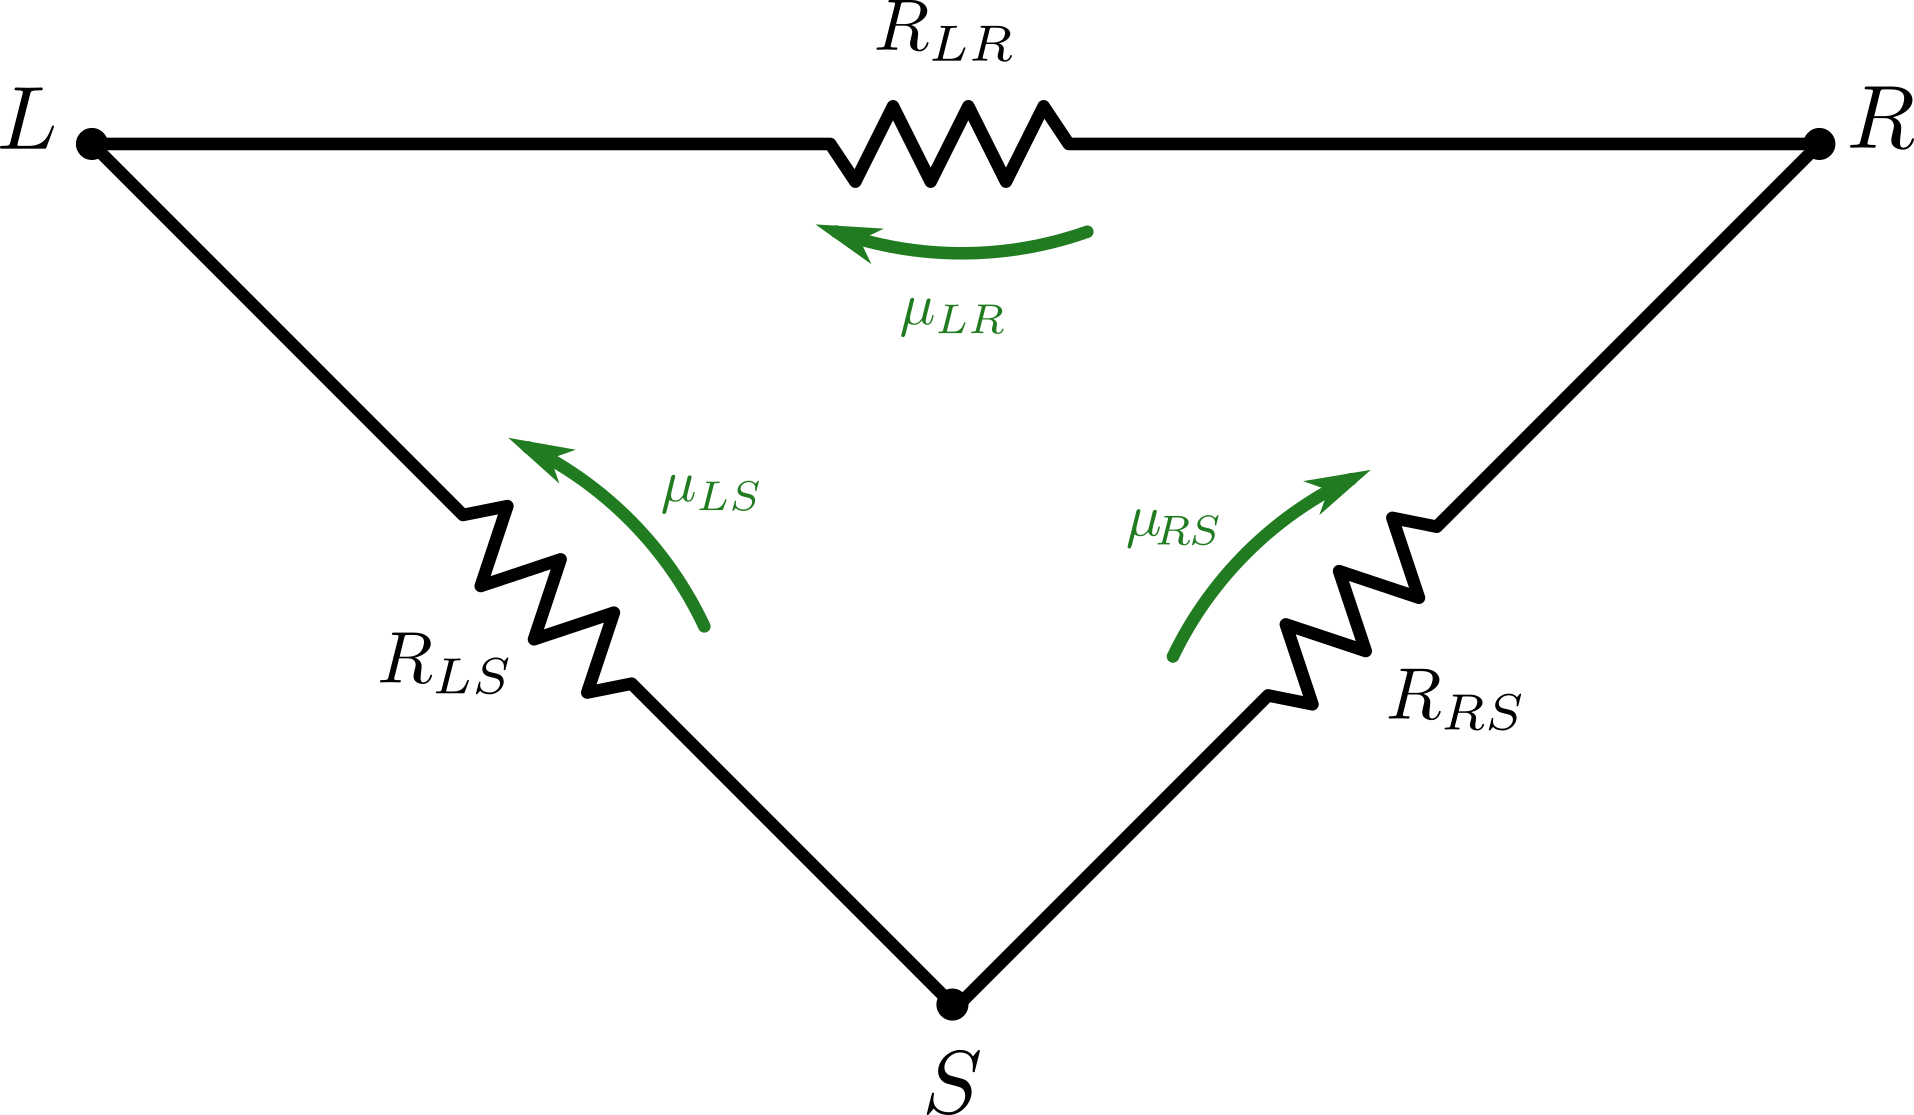
\includegraphics[scale=0.5]{triangle.png}
\caption{\label{fig1} A schematic resistor circuit illustrating the mapping of the three terminal nanostructure suggested by the authors.}
\end{figure}


In particular, $R_{LR,LR}$ is the local resistance which can be affected by the probe. The nonlocal resistances $R_{LR,RS}=-R_{LR,SR}, R_{LR,SL}=-R_{LR,LS}$ refer to the voltafe between the $\{R,S\}$ or $\{S,L\}$ terminals and the current flowing between $\{L,R\}$ electrodes. Since the energy of the system is conserved, $\Delta\mu_{LR}+\Delta\mu_{RS}+\Delta\mu_{SL}=0$, the local resistance $R_{LR,LR}$ is a linear combination of the two nonlocal resistances $R_{LR,SL}$ and $R_{LR,RS}$, $R_{LR,LR}=-R_{LR,SL}-R_{LR,RS}$. The local and nonlocal conductances are equivalent to the circuit conductances consisting of resistors $1/e\mathcal{L}_{ij,\mu}$ in a triangular geometry as illustrated in Fig. \ref{fig1}. In this way, the local conductance is a sum of the direct transmission between two ($L$ and $R$) terminals combined with an indirect one via additional voltage probe $S$:
\begin{align*}
\mathcal{G}_{LR,LR}\equiv\dfrac{1}{R_{LR,LR}}=\dfrac{eJ_{LR}}{\Delta\mu_{LR}}
\end{align*}
and using Eq. \eqref{Delta:muLR}, we obtain:
\begin{align*}
\mathcal{G}_{LR,LR}=
e\dfrac{\mathcal{L}_{LR,\mu} \mathcal{L}_{LS,\mu} +\mathcal{L}_{LR,\mu} \mathcal{L}_{RS,\mu} +\mathcal{L}_{LS,\mu} \mathcal{L}_{RS,\mu}}{\mathcal{L}_{RS,\mu}+\mathcal{L}_{LS,\mu}}
\end{align*}
and by divinding both numerator and denominator by $\mathcal{L}_{RS,\mu}\mathcal{L}_{LS,\mu}$ we obtain:
\begin{align*}
\mathcal{G}_{LR,LR}=
e\dfrac{\dfrac{\mathcal{L}_{LR,\mu} \mathcal{L}_{LS,\mu} + \mathcal{L}_{LR,\mu} \mathcal{L}_{RS,\mu} +\mathcal{L}_{LS,\mu} \mathcal{L}_{RS,\mu}}{\mathcal{L}_{RS,\mu}\mathcal{L}_{LS,\mu}}}{\dfrac{1}{\mathcal{L}_{RS,\mu}}+\dfrac{1}{\mathcal{L}_{LS,\mu}}}
\end{align*}
which can be put into the form
\begin{align*}
\mathcal{G}_{LR,LR}=
e\dfrac{\dfrac{\mathcal{L}_{LR,\mu} \mathcal{L}_{LS,\mu}}{\mathcal{L}_{RS,\mu}\mathcal{L}_{LS,\mu}}
+
\dfrac{\mathcal{L}_{LR,\mu} \mathcal{L}_{RS,\mu}}{\mathcal{L}_{RS,\mu}\mathcal{L}_{LS,\mu}}
+
1}{\dfrac{1}{\mathcal{L}_{RS,\mu}}+\dfrac{1}{\mathcal{L}_{LS,\mu}}}
\end{align*}
and by noticing some fractions may be simplified which leads to
\begin{align*}
\mathcal{G}_{LR,LR}=
e\dfrac{\dfrac{\mathcal{L}_{LR,\mu}}{\mathcal{L}_{RS,\mu}}
+
\dfrac{\mathcal{L}_{LR,\mu}}{\mathcal{L}_{LS,\mu}}
+
1}{\dfrac{1}{\mathcal{L}_{RS,\mu}}+\dfrac{1}{\mathcal{L}_{LS,\mu}}}.
\end{align*}

We can factor $\mathcal{L}_{LR,\mu}$ in the numerator to give:
\begin{align*}
\mathcal{G}_{LR,LR}=
e\dfrac{\mathcal{L}_{LR,\mu}\left[\dfrac{1}{\mathcal{L}_{RS,\mu}}
+
\dfrac{1}{\mathcal{L}_{LS,\mu}}\right]
+
1}{\dfrac{1}{\mathcal{L}_{RS,\mu}}+\dfrac{1}{\mathcal{L}_{LS,\mu}}}
\end{align*}
which leads to
\begin{align}\label{GLRLR}
\mathcal{G}_{LR,LR}=e\mathcal{L}_{LR,\mu}+
e\dfrac{
1}{\dfrac{1}{\mathcal{L}_{RS,\mu}}+\dfrac{1}{\mathcal{L}_{LS,\mu}}}.
\end{align}


Next, we determine the nonlocal conductance $\mathcal{G}_{LR,RS}$ which is given by:
\begin{align*}
\mathcal{G}_{LR,RS}=\dfrac{eJ_{LR}}{\Delta\mu_{RS}}
\end{align*}

From Eq. \eqref{Delta:muRS} we have:
\begin{align*}
\mathcal{G}_{LR,RS}=
-e\dfrac{
\mathcal{L}_{LR,\mu} \mathcal{L}_{LS,\mu} 
+\mathcal{L}_{LR,\mu} \mathcal{L}_{RS,\mu} 
+\mathcal{L}_{LS,\mu} \mathcal{L}_{RS,\mu}}{\mathcal{L}_{LS,\mu}},
\end{align*}
which may expressed as
\begin{align}\label{GLRRS}
\mathcal{G}_{LR,RS}=
-e\left[\mathcal{L}_{LR,\mu}
+\mathcal{L}_{RS,\mu}+\dfrac{
\mathcal{L}_{LR,\mu} \mathcal{L}_{RS,\mu} }{\mathcal{L}_{LS,\mu}}\right].
\end{align}

Next, we obtain the conductance $\mathcal{G}_{LR,LS}$, by using the definition:
\begin{align*}
\mathcal{G}_{LR,LS}=\dfrac{eJ_{LR}}{\Delta\mu_{LS}},
\end{align*}
and by using Eq. \eqref{Delta:muLS}
\begin{align*}
\mathcal{G}_{LR,LS}
=
e\dfrac{\mathcal{L}_{LR,\mu} \mathcal{L}_{LS,\mu} + \mathcal{L}_{LR,\mu} \mathcal{L}_{RS,\mu} + \mathcal{L}_{LS,\mu} \mathcal{L}_{RS,\mu}}{\mathcal{L}_{RS,\mu}}
\end{align*}
which may be written as, 
\begin{align}\label{GLRLS}
\mathcal{G}_{LR,LS}
=
e\left[\mathcal{L}_{LR,\mu} + \mathcal{L}_{LS,\mu} +\dfrac{\mathcal{L}_{LR,\mu} \mathcal{L}_{LS,\mu}}{\mathcal{L}_{RS,\mu}}\right].
\end{align}


\subsection{Demonstration of Eq. (B6)}

In order to determine the $\mathcal{L}$ coefficients in terms of te resistances, we need to determine the expression for $R_{RS,LS}$ which is defined by taking the $L$-lead as a probe. In this case, we set $J_{L}=0$ and take $J_{R}=-J_{S}=J_{RS}$ in analogy to the previous definitions. By using Eqs. \eqref{delta:mu:L}, \eqref{delta:mu:R} and \eqref{delta:mu:S}, we can calculate the chemical potential differences among the leads, i.e., $\Delta\mu_{LS}$, $\Delta\mu_{RS}$ and $\Delta\mu_{LR}$ in a similar way we have obtained the previous calculations. By substituting $J_{L}=0$, $J_{R}=-J_{S}=J_{RS}$ in Eqs. \eqref{delta:mu:L}, \eqref{delta:mu:R} and \eqref{delta:mu:S} we have:
\begin{widetext}
\begin{align}\label{deltaL:mu:L}
\delta_{L}\mu_{L}
=\dfrac{1}{D_{\mu}}
\{
\mathcal{L}_{LR,\mu}\mathcal{L}_{SL,\mu}
-
\mathcal{L}_{LR,\mu}\mathcal{L}_{LS,\mu}
-
\mathcal{L}_{LR,\mu}\mathcal{L}_{RS,\mu}
+
\mathcal{L}_{LR,\mu}\mathcal{L}_{SR,\mu}
-
\mathcal{L}_{LS,\mu}\mathcal{L}_{RS,\mu}
+
\mathcal{L}_{LS,\mu}\mathcal{L}_{SR,\mu}
\}J_{RS},
\end{align}  
\begin{align}\label{deltaL:mu:S}
\delta_{L}\mu_{S}
=\dfrac{1}{D_{\mu}}
\{
\mathcal{L}_{LR,\mu}\mathcal{L}_{SR,\mu}
-
\mathcal{L}_{LR,\mu}\mathcal{L}_{SL,\mu}
-
\mathcal{L}_{LR,\mu}\mathcal{L}_{LS,\mu}
-
\mathcal{L}_{LR,\mu}\mathcal{L}_{RS,\mu}
+
\mathcal{L}_{LS,\mu}\mathcal{L}_{SR,\mu}
-
\mathcal{L}_{LS,\mu}\mathcal{L}_{RS,\mu}
\}J_{RS},
\end{align} 
\begin{align}\label{deltaL:mu:R}
\delta_{L}\mu_{R}
=\dfrac{1}{D_{\mu}}
\{
\mathcal{L}_{LR,\mu}\mathcal{L}_{SL,\mu}
+
\mathcal{L}_{LR,\mu}\mathcal{L}_{SR,\mu}
-
\mathcal{L}_{LR,\mu}\mathcal{L}_{LS,\mu}
-
\mathcal{L}_{LR,\mu}\mathcal{L}_{RS,\mu}
+2
\mathcal{L}_{SL,\mu}\mathcal{L}_{LS,\mu}
+
\mathcal{L}_{SR,\mu}\mathcal{L}_{LS,\mu}
-
\mathcal{L}_{LS,\mu}\mathcal{L}_{RS,\mu}
\}J_{RS}.
\end{align}

Next, we calculate the chemical potencial differences as follows:
\begin{align*}
\Delta_{L}\mu_{LS}
=
\delta_{L}\mu_{L}-\delta_{L}\mu_{S}
=
\dfrac{1}{D_{\mu}}
\{
\mathcal{L}_{LR,\mu}\mathcal{L}_{SL,\mu}
-
\mathcal{L}_{LR,\mu}\mathcal{L}_{LS,\mu}
-
\mathcal{L}_{LR,\mu}\mathcal{L}_{RS,\mu}
+
\mathcal{L}_{LR,\mu}\mathcal{L}_{SR,\mu}
-
\mathcal{L}_{LS,\mu}\mathcal{L}_{RS,\mu}
+
\mathcal{L}_{LS,\mu}\mathcal{L}_{SR,\mu}
\\
-
\mathcal{L}_{LR,\mu}\mathcal{L}_{SR,\mu}
+
\mathcal{L}_{LR,\mu}\mathcal{L}_{SL,\mu}
+
\mathcal{L}_{LR,\mu}\mathcal{L}_{LS,\mu}
+
\mathcal{L}_{LR,\mu}\mathcal{L}_{RS,\mu}
-
\mathcal{L}_{LS,\mu}\mathcal{L}_{SR,\mu}
+
\mathcal{L}_{LS,\mu}\mathcal{L}_{RS,\mu}
\}J_{RS}
\end{align*}
\end{widetext}
which leads to
\begin{align}\label{LDeltaLS:eq1}
\Delta_{L}\mu_{LS}
=
\dfrac{\mathcal{L}_{LR,\mu}}{\mathcal{L}_{LR,\mu} \mathcal{L}_{LS,\mu} +\mathcal{L}_{LR,\mu} \mathcal{L}_{RS,\mu}+\mathcal{L}_{LS,\mu} \mathcal{L}_{RS,\mu} }
J_{RS}.
\end{align}

% Next, we calculate the chemical potential between $R$ and $S$ leads:
% \begin{widetext}
% \begin{multline*}
% \Delta_{L}\mu_{RS}=\delta_{L}\mu_{R}-\delta_{L}\mu_{S}=
% \\=
% \dfrac{1}{D_{\mu}}
% \{
% \mathcal{L}_{LR,\mu}\mathcal{L}_{SL,\mu}
% +
% \mathcal{L}_{LR,\mu}\mathcal{L}_{SR,\mu}
% -
% \mathcal{L}_{LR,\mu}\mathcal{L}_{LS,\mu}
% -
% \mathcal{L}_{LR,\mu}\mathcal{L}_{RS,\mu}
% +2
% \mathcal{L}_{SL,\mu}\mathcal{L}_{LS,\mu}
% +
% \mathcal{L}_{SR,\mu}\mathcal{L}_{LS,\mu}
% -
% \mathcal{L}_{LS,\mu}\mathcal{L}_{RS,\mu}
% \\
% -\mathcal{L}_{LR,\mu}\mathcal{L}_{SR,\mu}
% +
% \mathcal{L}_{LR,\mu}\mathcal{L}_{SL,\mu}
% +
% \mathcal{L}_{LR,\mu}\mathcal{L}_{LS,\mu}
% +
% \mathcal{L}_{LR,\mu}\mathcal{L}_{RS,\mu}
% -
% \mathcal{L}_{LS,\mu}\mathcal{L}_{SR,\mu}
% +
% \mathcal{L}_{LS,\mu}\mathcal{L}_{RS,\mu}
% \}J_{RS}
% \end{multline*}    
% \end{widetext}
% which leads to
% \begin{align}\label{LDeltaRS:eq1}
% \Delta_{L}\mu_{RS}=\dfrac{(\mathcal{L}_{LS,\mu}+\mathcal{L}_{LR,\mu})}{\mathcal{L}_{LR,\mu} \mathcal{L}_{LS,\mu} +\mathcal{L}_{LR,\mu} \mathcal{L}_{RS,\mu} +\mathcal{L}_{LS,\mu} \mathcal{L}_{RS,\mu}}J_{RS}.
% \end{align}


Next, we determine the resistance $R_{RS,LS}$ which is defined as follows:
\begin{align*}
R_{RS,LS}=\dfrac{\Delta\mu_{LS}}{eJ_{RS}}
\end{align*}
and, by using Eq. \eqref{LDeltaLS:eq1}, we have:
\begin{align*}
\Delta_{L}\mu_{LS}
=
\dfrac{\mathcal{L}_{LR,\mu}}{\mathcal{L}_{LR,\mu} \mathcal{L}_{LS,\mu} +\mathcal{L}_{LR,\mu} \mathcal{L}_{RS,\mu}+\mathcal{L}_{LS,\mu} \mathcal{L}_{RS,\mu}}J_{RS}.
\end{align*}

We can express the conductance in terms of the coefficients:
\begin{align}\label{GRSLS:eq1}
\mathcal{G}_{RS,LS}=e\left[\mathcal{L}_{LS,\mu}+\mathcal{L}_{RS,\mu}+\dfrac{\mathcal{L}_{LS,\mu} \mathcal{L}_{RS,\mu}}{\mathcal{L}_{LR,\mu}}\right].
\end{align}


By using Eq. \eqref{GRSLS:eq1} and the previous defintions for $\mathcal{G}_{LR,RS}$ and $\mathcal{G}_{LR,RS}$ we can form the following system of equations:
\begin{align*}
\mathcal{G}_{LR,LS}=\dfrac{1}{{R}_{LR,LS}}
&=
+e\left[\mathcal{L}_{LR,\mu} + \mathcal{L}_{LS,\mu} +\dfrac{\mathcal{L}_{LR,\mu} \mathcal{L}_{LS,\mu}}{\mathcal{L}_{RS,\mu}}\right],
\\
\mathcal{G}_{LR,RS}=\dfrac{1}{{R}_{LR,RS}}
&=
-e\left[\mathcal{L}_{LR,\mu}
+\mathcal{L}_{RS,\mu}+\dfrac{
\mathcal{L}_{LR,\mu} \mathcal{L}_{RS,\mu} }{\mathcal{L}_{LS,\mu}}\right],
\\
\mathcal{G}_{RS,LS}=\dfrac{1}{{R}_{RS,LS}}&=
+e\left[\mathcal{L}_{LS,\mu}+\mathcal{L}_{RS,\mu}+\dfrac{\mathcal{L}_{LS,\mu} \mathcal{L}_{RS,\mu}}{\mathcal{L}_{LR,\mu}}\right].
\end{align*}

These equations may be written as follows:
\begin{align}\label{Rs:definitions}
R_{LR,LS}
=
\dfrac{\mathcal{L}_{RS,\mu}}{eD_{L}},
\quad
R_{LR,RS}=-\dfrac{\mathcal{L}_{LS,\mu}}{eD_{L}},
\quad
R_{RS,LS}=\dfrac{\mathcal{L}_{LR,\mu}}{eD_{L}}
\end{align}
where we have defined,
$D_{L}=\mathcal{L}_{LR,\mu}\mathcal{L}_{RS,\mu} + \mathcal{L}_{LS,\mu}\mathcal{L}_{RS,\mu} +\mathcal{L}_{LR,\mu}\mathcal{L}_{LS,\mu}$.

Let's calculate the following quantity, $D_{R}$:
\begin{widetext}
\begin{multline}\label{DR:def}
D_{R}=R_{RS,LS}R_{LR,LS}
-
R_{LR,LS}R_{LR,RS}
-
R_{LR,RS}R_{RS,LS}
\\=
\dfrac{\mathcal{L}_{LR,\mu}}{eD_{L}}
\dfrac{\mathcal{L}_{RS,\mu}}{eD_{L}}
+
\dfrac{\mathcal{L}_{RS,\mu}}{eD_{L}}
\dfrac{\mathcal{L}_{LS,\mu}}{eD_{L}}
+
\dfrac{\mathcal{L}_{LS,\mu}}{eD_{L}}
\dfrac{\mathcal{L}_{LR,\mu}}{eD_{L}}
=
\dfrac{D_{L}}{e^{2}D^{2}_{L}}=\dfrac{1}{e^{2}D_{L}}
\end{multline}
\end{widetext}
which leads to:
\begin{align}\label{DR:def:2}
eD_{R}=\dfrac{1}{eD_{L}}.
\end{align}
\clearpage
Next, we replace $D_{L}$ by $D_{R}$ in Eqs. \eqref{Rs:definitions} which leads to,
\begin{align*}
R_{LR,LS}
&=
\mathcal{L}_{RS,\mu}eD_{R},
\\
R_{LR,RS}
&=-\mathcal{L}_{LS,\mu}eD_{R}
\\
R_{RS,LS}
&=\mathcal{L}_{LR,\mu}eD_{R}
\end{align*}
which allows us to express the coefficients in terms of the resistances, which may be measured in experiments. 
\begin{align}\label{LRS:exp}
\mathcal{L}_{RS,\mu}=\dfrac{R_{LR,LS}}{eD_{R}},
\end{align}
\begin{align}\label{LLS:exp}
\mathcal{L}_{LS,\mu}=-\dfrac{R_{LR,RS}}{eD_{R}}
\end{align}
\begin{align}\label{LLR:exp}
\mathcal{L}_{LR,\mu}=\dfrac{R_{RS,LS}}{eD_{R}}
\end{align}
\section{APPENDIX B: Using $S$ as a probe}

Let's use Eq. (2) along with the assumption the $S$ leads is a probe. In this case, we have:
\begin{align}\label{JL}
J_{L}&=
(\mathcal{L}_{LS,\mu}+\mathcal{L}_{LR,\mu} )\delta\mu_{L}
-\mathcal{L}_{LS,\mu}\delta\mu_{S}
-\mathcal{L}_{LR,\mu}\delta\mu_{R}
\\\label{JS}
J_{S}&=
-\mathcal{L}_{SL,\mu}\delta\mu_{L}
+
(\mathcal{L}_{SL,\mu}+\mathcal{L}_{SR,\mu})\delta\mu_{S}
-
\mathcal{L}_{SR,\mu}\delta\mu_{R}
\\\label{JR}
J_{R}&= 
-\mathcal{L}_{RL,\mu}\delta\mu_{L} 
-\mathcal{L}_{RS,\mu}\delta\mu_{S}
+
(\mathcal{L}_{RL,\mu}+\mathcal{L}_{RS,\mu})\delta\mu_{R}
\end{align}

by using the condition $J_{S}=0$, the superconductor lead as a probe, then we can eliminate $\delta\mu_{S}$ from the equations above. In fact, from the second equation we have:
\begin{align*}
J_{S}&=0=
-\mathcal{L}_{SL,\mu}\delta\mu_{L}
+
(\mathcal{L}_{SL,\mu}+\mathcal{L}_{SR,\mu})\delta\mu_{S}
-
\mathcal{L}_{SR,\mu}\delta\mu_{R}
\end{align*}
which allows us to write:
\begin{align}\label{delta:muS}
\delta\mu_{S}
=
\dfrac{\mathcal{L}_{SL,\mu}\delta\mu_{L}+\mathcal{L}_{SR,\mu}\delta\mu_{R}}{\mathcal{L}_{SL,\mu}+\mathcal{L}_{SR,\mu}}
\end{align}
\begin{widetext}
and by plugging this into Eqs. for $J_{L}$ and $J_{R}$, we have:
\begin{align*}
J_{L}&=
(\mathcal{L}_{LS,\mu}+\mathcal{L}_{LR,\mu})\delta\mu_{L}
-\mathcal{L}_{LS,\mu}\left[\dfrac{\mathcal{L}_{SL,\mu}\delta\mu_{L}+\mathcal{L}_{SR,\mu}\delta\mu_{R}}{\mathcal{L}_{SL,\mu}+\mathcal{L}_{SR,\mu}}\right]
-\mathcal{L}_{LR,\mu}\delta\mu_{R}
\end{align*}
which leads to
\begin{align*}
J_{L}&=
\dfrac{(\mathcal{L}_{LS,\mu}+\mathcal{L}_{LR,\mu})(\mathcal{L}_{SL,\mu}+\mathcal{L}_{SR,\mu})}{\mathcal{L}_{SL,\mu}+\mathcal{L}_{SR,\mu}}\delta\mu_{L}
-
\dfrac{\mathcal{L}_{LS,\mu}\mathcal{L}_{SL,\mu}}{\mathcal{L}_{SL,\mu}+\mathcal{L}_{SR,\mu}}\delta\mu_{L}
-
\dfrac{\mathcal{L}_{LS,\mu}\mathcal{L}_{SR,\mu}}{\mathcal{L}_{SL,\mu}+\mathcal{L}_{SR,\mu}}\delta\mu_{R}
-
\mathcal{L}_{LR,\mu}\delta\mu_{R}
\end{align*}
which leads to
\begin{align*}
J_{L}&=
\dfrac{(\mathcal{L}_{LS,\mu}+\mathcal{L}_{LR,\mu})(\mathcal{L}_{SL,\mu}+\mathcal{L}_{SR,\mu})-\mathcal{L}_{LS,\mu}\mathcal{L}_{SL,\mu}}{\mathcal{L}_{SL,\mu}+\mathcal{L}_{SR,\mu}}\delta\mu_{L}
-\left[
\dfrac{\mathcal{L}_{LS,\mu}\mathcal{L}_{SR,\mu}+\mathcal{L}_{LR,\mu}(\mathcal{L}_{SL,\mu}+\mathcal{L}_{SR,\mu})}{\mathcal{L}_{SL,\mu}+\mathcal{L}_{SR,\mu}}\delta\mu_{R}
\right]
\end{align*}
\begin{multline*}
J_{L}=
\dfrac{\mathcal{L}_{LS,\mu}\mathcal{L}_{SL,\mu}
+
\mathcal{L}_{LS,\mu}\mathcal{L}_{SR,\mu}
+
\mathcal{L}_{LR,\mu}\mathcal{L}_{SL,\mu}
+
\mathcal{L}_{LR,\mu}\mathcal{L}_{SR,\mu}-\mathcal{L}_{LS,\mu}\mathcal{L}_{SL,\mu}}{\mathcal{L}_{SL,\mu}+\mathcal{L}_{SR,\mu}}\delta\mu_{L}
\\-\left[
\dfrac{\mathcal{L}_{LS,\mu}\mathcal{L}_{SR,\mu}+\mathcal{L}_{LR,\mu}(\mathcal{L}_{SL,\mu}+\mathcal{L}_{SR,\mu})}{\mathcal{L}_{SL,\mu}+\mathcal{L}_{SR,\mu}}
\right]\delta\mu_{R}
\end{multline*}
and performing some simplifications, we have:
\begin{align*}
J_{L}=
\dfrac{
\mathcal{L}_{LS,\mu}\mathcal{L}_{SR,\mu}
+
\mathcal{L}_{LR,\mu}\mathcal{L}_{SL,\mu}
+
\mathcal{L}_{LR,\mu}\mathcal{L}_{SR,\mu}}{\mathcal{L}_{SL,\mu}+\mathcal{L}_{SR,\mu}}\delta\mu_{L}
-\left[
\dfrac{\mathcal{L}_{LS,\mu}\mathcal{L}_{SR,\mu}+\mathcal{L}_{LR,\mu}\mathcal{L}_{SL,\mu}+\mathcal{L}_{LR,\mu}\mathcal{L}_{SR,\mu}}{\mathcal{L}_{SL,\mu}+\mathcal{L}_{SR,\mu}}
\right]\delta\mu_{R}
\end{align*} 
and by defining, 
\begin{align*}
D_{L}=\mathcal{L}_{LS,\mu}\mathcal{L}_{SR,\mu}+\mathcal{L}_{LR,\mu}\mathcal{L}_{SL,\mu}+\mathcal{L}_{LR,\mu}\mathcal{L}_{SR,\mu}
\end{align*}
\end{widetext}
we can write the equation above as:
\begin{align*}
J_{L}=\dfrac{D_{L}}{\mathcal{L}_{SL,\mu}+\mathcal{L}_{SR,\mu}}(\delta\mu_{L}-\delta\mu_{R})
\end{align*}
which can be put into the form:
\begin{align*}
J_{L}=\dfrac{D_{L}}{\mathcal{L}_{SL,\mu}+\mathcal{L}_{SR,\mu}}\Delta\mu_{LR}
\end{align*}
which leads to:
\begin{align}\label{Delta:mu:LR}
\Delta\mu_{LR}=\dfrac{\mathcal{L}_{SL,\mu}+\mathcal{L}_{SR,\mu}}{D_{L}}J_{LR}.
\end{align} 
where $J_{LR}=J_{L}=-J_{R}$ from the paper. We notice that  Eq. \eqref{Delta:mu:LR} corresponds to Eq. (B1) from the paper (we must assume the time-reversal symmetry so the coefficient are symetric under exchanging of index).

The other equations in (B1) are determined by using Eq. \eqref{Delta:mu:LR}

We should obtain the same result if we substitute Eq. \eqref{delta:muS} into Eq. \eqref{JR} \footnote{Indeed, let's substitute Eq. \eqref{delta:muS} into Eq. \eqref{JR}:
\begin{align*}
J_{R}&= 
-\mathcal{L}_{RL,\mu}\delta\mu_{L} 
-\mathcal{L}_{RS,\mu}\left[\dfrac{\mathcal{L}_{SL,\mu}\delta\mu_{L}+\mathcal{L}_{SR,\mu}\delta\mu_{R}}{\mathcal{L}_{SL,\mu}+\mathcal{L}_{SR,\mu}}\right]
+
(\mathcal{L}_{RL,\mu}+\mathcal{L}_{RS,\mu})\delta\mu_{R}
\end{align*}

\begin{align*}
J_{R}&= 
-\mathcal{L}_{RL,\mu}\delta\mu_{L} 
-
\dfrac{\mathcal{L}_{RS,\mu}\mathcal{L}_{SL,\mu}}{\mathcal{L}_{SL,\mu}+\mathcal{L}_{SR,\mu}}\delta\mu_{L}
-
\dfrac{\mathcal{L}_{RS,\mu}\mathcal{L}_{SR,\mu}}{\mathcal{L}_{SL,\mu}+\mathcal{L}_{SR,\mu}}\delta\mu_{R}
+
(\mathcal{L}_{RL,\mu}+\mathcal{L}_{RS,\mu})\delta\mu_{R}
\end{align*}
\begin{multline*}
J_{R}= 
-\left[
\dfrac{\mathcal{L}_{RL,\mu}(\mathcal{L}_{SL,\mu}+\mathcal{L}_{SR,\mu})+\mathcal{L}_{RS,\mu}\mathcal{L}_{SL,\mu}}{\mathcal{L}_{SL,\mu}+\mathcal{L}_{SR,\mu}}\right]\delta\mu_{L}
\\+\left[
\dfrac{-\mathcal{L}_{RS,\mu}\mathcal{L}_{SR,\mu}+(\mathcal{L}_{SL,\mu}+\mathcal{L}_{SR,\mu})(\mathcal{L}_{RL,\mu}+\mathcal{L}_{RS,\mu})}{\mathcal{L}_{SL,\mu}+\mathcal{L}_{SR,\mu}}\right]\delta\mu_{R}
\end{multline*}

\begin{multline*}
J_{R}= 
-\left[
\dfrac{\mathcal{L}_{RL,\mu}\mathcal{L}_{SL,\mu}+\mathcal{L}_{RL,\mu}\mathcal{L}_{SR,\mu}+\mathcal{L}_{RS,\mu}\mathcal{L}_{SL,\mu}}{\mathcal{L}_{SL,\mu}+\mathcal{L}_{SR,\mu}}\right]\delta\mu_{L}
\\+\left[
\dfrac{-\mathcal{L}_{RS,\mu}\mathcal{L}_{SR,\mu}+\mathcal{L}_{SL,\mu}\mathcal{L}_{RL,\mu}
+\mathcal{L}_{SL,\mu}\mathcal{L}_{RS,\mu}
+\mathcal{L}_{SR,\mu}\mathcal{L}_{RL,\mu}
+\mathcal{L}_{SR,\mu}\mathcal{L}_{RS,\mu}}{\mathcal{L}_{SL,\mu}+\mathcal{L}_{SR,\mu}}\right]\delta\mu_{R}
\end{multline*}

\begin{multline*}
J_{R}= 
-\left[
\dfrac{\mathcal{L}_{RL,\mu}\mathcal{L}_{SL,\mu}+\mathcal{L}_{RL,\mu}\mathcal{L}_{SR,\mu}+\mathcal{L}_{RS,\mu}\mathcal{L}_{SL,\mu}}{\mathcal{L}_{SL,\mu}+\mathcal{L}_{SR,\mu}}\right]\delta\mu_{L}
\\+\left[
\dfrac{
\mathcal{L}_{SL,\mu}\mathcal{L}_{RL,\mu}
+\mathcal{L}_{SL,\mu}\mathcal{L}_{RS,\mu}
+\mathcal{L}_{SR,\mu}\mathcal{L}_{RL,\mu}
}{\mathcal{L}_{SL,\mu}+\mathcal{L}_{SR,\mu}}\right]\delta\mu_{R}
\end{multline*}
and by using the definition of $D_{L}$ we have:
\begin{align*}
J_{R}=\dfrac{D_{L}}{\mathcal{L}_{SL,\mu}+\mathcal{L}_{SR,\mu}}(-\delta\mu_{L}+\delta\mu_{R})=-\dfrac{D_{L}}{\mathcal{L}_{SL,\mu}+\mathcal{L}_{SR,\mu}}\Delta\mu_{LR}
\end{align*}
which leads to:
\begin{align*}
\Delta\mu_{LR}=\dfrac{\mathcal{L}_{SL,\mu}+\mathcal{L}_{SR,\mu}}{D_{L}}J_{LR}
\end{align*} which is indeed Eq. \eqref{Delta:mu:LR}.}. Next, we calculate:
\begin{align*}
\Delta\mu_{LS}&=\delta\mu_{L}-\delta\mu_{S}
=
\delta\mu_{L}-\dfrac{\mathcal{L}_{SL,\mu}\delta\mu_{L}+\mathcal{L}_{SR,\mu}\delta\mu_{R}}{\mathcal{L}_{SL,\mu}+\mathcal{L}_{SR,\mu}}
\\
&=\delta\mu_{L}\dfrac{(\mathcal{L}_{SL,\mu}+\mathcal{L}_{SR,\mu})}{\mathcal{L}_{SL,\mu}+\mathcal{L}_{SR,\mu}}-\dfrac{\mathcal{L}_{SL,\mu}\delta\mu_{L}+\mathcal{L}_{SR,\mu}\delta\mu_{R}}{\mathcal{L}_{SL,\mu}+\mathcal{L}_{SR,\mu}}
\end{align*}
which leads to
\begin{align*}
\Delta\mu_{LS}
&=\dfrac{\mathcal{L}_{SR,\mu}}{\mathcal{L}_{SL,\mu}+\mathcal{L}_{SR,\mu}}(\delta\mu_{L}-\delta\mu_{R})
\end{align*}
then, we have:
\begin{align}\label{Delta:mu:LS:intermed}
\Delta\mu_{LS}
&=\dfrac{\mathcal{L}_{SR,\mu}}{\mathcal{L}_{SL,\mu}+\mathcal{L}_{SR,\mu}}\Delta\mu_{LR}.
\end{align}

By substituting Eq. \eqref{Delta:mu:LR} into Eq. \eqref{Delta:mu:LS:intermed} we obtain:
\begin{align}\label{Delta:mu:LS:intermed}
\Delta\mu_{LS}
&=\dfrac{\mathcal{L}_{SR,\mu}}{\mathcal{L}_{SL,\mu}+\mathcal{L}_{SR,\mu}}\dfrac{\mathcal{L}_{SL,\mu}+\mathcal{L}_{SR,\mu}}{D_{L}}J_{LR},
\end{align}
which leads to
\begin{align}\label{Delta:mu:LS}
\Delta\mu_{LS}
&=\dfrac{\mathcal{L}_{SR,\mu}}{D_{L}}J_{LR}.
\end{align}

Next, we calculate $\Delta\mu_{RS}$ as follows:
\begin{align*}
\Delta\mu_{RS}=\delta\mu_{R}-\delta\mu_{S}
=
\delta\mu_{R}-\delta\mu_{L}+\delta\mu_{L}-\delta\mu_{S}
=
-\Delta\mu_{LR}+\Delta\mu_{LS}
\end{align*}
and by using \eqref{Delta:mu:LR} and \eqref{Delta:mu:LS} we obtain:
\begin{align*}
\Delta\mu_{RS}
=
-\dfrac{(\mathcal{L}_{SL,\mu}+\mathcal{L}_{SR,\mu})}{D_{L}}J_{LR}+\dfrac{\mathcal{L}_{SR,\mu}}{D_{L}}J_{LR}
\end{align*}
which leads to 
\begin{align}\label{Delta:mu:RS}
\Delta\mu_{RS}
=
-\dfrac{\mathcal{L}_{SL,\mu}}{D_{L}}J_{LR}.
\end{align}
%PHYSICS LETTERS A PASSWORD AND LOGIN:
%LOGIN:ezcostta@gmail.com
%PASSWORD: Brasil*1981


\end{document}
